\documentclass[12pt,a4paper]{ctexart}
\usepackage[top=2.5cm,bottom=2.5cm,left=2.5cm,right=2.5cm]{geometry}
\usepackage{amsmath,amssymb,amsfonts}
\usepackage{graphicx}
\usepackage{booktabs,array}
\usepackage{caption,float}
\usepackage{xcolor}

\graphicspath{{../figures/}}

\title{\textbf{古代玻璃制品的成分分析与鉴别}}
\author{}
\date{}

\begin{document}
\maketitle

\begin{abstract}
\noindent 本文针对古代玻璃制品风化与其化学成分之间的关系，综合运用统计学检验、组成数据分析(CoDa)、层次聚类、随机森林分类和排列检验等方法，建立了从风化分析到类别鉴别、再到成分关联挖掘的完整建模体系。

\textbf{问题一}：通过卡方检验和Cramer's V效应量分析，发现玻璃风化与玻璃类型($p=0.020$, $V=0.307$)和纹饰类型($p=0.027$, $V=0.333$)存在显著关联。在CLR变换框架下，利用Welch $t$检验结合Holm-Bonferroni多重检验校正，识别了各玻璃类型中风化敏感的化学成分。基于不移动元素Al$_2$O$_3$的归一化方法，建立了风化前成分预测模型，在11对校准样本上的平均绝对误差(MAE)为5.73\%。

\textbf{问题二}：通过随机森林、$t$检验和互信息三种方法的共识排名，确定PbO、BaO、K$_2$O、SrO和SiO$_2$为判别高钾玻璃与铅钡玻璃的关键元素。基于CLR变换后的Ward层次聚类，将高钾玻璃划分为2个亚类(轮廓系数0.269)，铅钡玻璃划分为4个亚类(轮廓系数0.214)。Bootstrap重采样验证显示聚类稳定性良好(中位ARI $>$ 0.55)。

\textbf{问题三}：采用$k$-近邻($k=3,5$)和随机森林两种分类器对8个未知文物进行分类，A1、A6、A7鉴定为高钾玻璃，A2--A5、A8鉴定为铅钡玻璃。5\%扰动下的分类稳定性达98.00\%。

\textbf{问题四}：基于Aitchison几何框架，计算了组成变异矩阵并采用排列检验($n=5000$)比较了不同玻璃类型的相关结构差异，发现高钾与铅钡玻璃的化学成分关联结构存在显著差异($p=0.0032$)，反映了两种玻璃在制作工艺和原料来源上的本质区别。

\textbf{关键词}：组成数据分析；CLR变换；层次聚类；随机森林；排列检验；古代玻璃
\end{abstract}

\newpage
\tableofcontents
\newpage

\section{问题重述}
\subsection{问题背景}

丝绸之路是古代中西方文化交流的通道，其中玻璃是早期贸易往来的宝贵物证。我国古代玻璃吸收外来技术后在本土取材制作，因此与外来玻璃制品外观相似但化学成分不同。玻璃的主要原料为石英砂(SiO$_2$)，炼制时需添加助熔剂(草木灰、天然泡碱、铅矿石等)和稳定剂(石灰石→CaO)。不同的助熔剂决定了玻璃的主要化学特征：铅钡玻璃以PbO和BaO含量高为特征，被认为是我国独创的玻璃品种；钾玻璃以K$_2$O含量高为特征，流行于岭南及东南亚地区。

古代玻璃在埋藏环境中极易风化，风化过程中内部元素与环境元素进行大量交换，导致成分比例发生变化，从而影响对类别的正确判断。因此，需要建立科学的分析方法，探究风化规律，并在此基础上对玻璃文物进行准确分类和成分关联分析。

\subsection{问题提出}

\textbf{问题1}：分析玻璃文物表面风化与玻璃类型、纹饰和颜色的关系；结合玻璃类型，分析有无风化化学成分含量的统计规律；根据风化点检测数据，预测风化前的化学成分含量。

\textbf{问题2}：分析高钾玻璃和铅钡玻璃的分类规律；选择合适的化学成分对每类玻璃进行亚类划分，给出划分方法及结果，分析分类结果的合理性和敏感性。

\textbf{问题3}：对未知类别玻璃文物(附件表单3)的化学成分进行分析，鉴别其所属类型，并对分类结果进行敏感性分析。

\textbf{问题4}：分析不同类别玻璃文物样品化学成分之间的关联关系，比较不同类别之间化学成分关联关系的差异性。

\section{模型假设}

\begin{enumerate}
    \item 玻璃成分的空白值表示该成分含量低于检测仪器的检出限，而非完全不存在。
    \item 成分比例累加和在85\%--105\%之间的数据视为有效数据，其余视为检测误差。
    \item 风化过程主要是元素的淋失或富集，不改变Al$_2$O$_3$等不移动元素在整体中的相对位置。
    \item 同一墓葬出土的不同文物样品间相互独立，不存在交叉污染。
    \item 文物采样点(部位1/部位2)的化学成分差异反映了该文物不同区域的客观差异。
\end{enumerate}

\section{符号说明}

\begin{table}[H]
\centering
\caption{主要符号说明}
\begin{tabular}{c|l|c|l}
\toprule
\textbf{符号} & \textbf{含义} & \textbf{符号} & \textbf{含义} \\
\midrule
$\mathbf{x} = (x_1,\dots,x_{12})$ & 12种化学成分比例向量 & $\text{clr}(\mathbf{x})$ & 中心对数比变换 \\
$\mathcal{G}(\mathbf{x})$ & 几何均值 & $g_{jk}$ & 成分$j,k$的对数比方差 \\
$\chi^2$ & 卡方统计量 & $V$ & Cramer's V效应量 \\
$\delta$ & Cohen's $d$效应量 & $d_{\text{holm}}$ & Holm-Bonferroni校正后$p$值 \\
$\text{EF}$ & Al$_2$O$_3$富集因子 & $\tau_{ij}$ & 组成变异矩阵元素 \\
$k$ & 聚类数/最近邻邻居数 & $T$ & 排列检验统计量 \\
\bottomrule
\end{tabular}
\end{table}

\section{数据预处理}

\subsection{数据来源与结构}

附件包含三个表单：
\begin{itemize}
    \item \textbf{表单1}：58件文物的基本信息，包括文物编号、纹饰(A/B/C)、类型(高钾/铅钡)、颜色、表面风化状态。
    \item \textbf{表单2}：已分类玻璃文物的化学成分比例(14种氧化物)，共69条采样点记录。每个采样点记录了SiO$_2$、Na$_2$O、K$_2$O等14种氧化物的重量百分比。
    \item \textbf{表单3}：8件未分类玻璃文物的化学成分比例，含表面风化状态，与表单2化学成分字段一致。
\end{itemize}

\subsection{数据清洗与预处理}

\textbf{(1) 化学成分筛选}：SnO$_2$和SO$_2$缺失率分别达到89.9\%和88.4\%，无法支持任何有效统计推断，予以剔除。最终保留12种化学成分用于全部建模分析。

\textbf{(2) 缺失值处理}：Na$_2$O在高钾玻璃中系统性缺失(检出限以下)，K$_2$O在铅钡玻璃中常缺失。采用领域知识指导的填补策略：对于玻璃类型确定的样本，使用该类玻璃中的最小非零值的一半作为检出限替代值。其余缺失采用各成分的半最小非零值填补。

\textbf{(3) 零值处理}：A8样品中含Na$_2$O=0、MgO=0等零值。在进行对数变换前，采用乘性替换策略，将所有零值替换为各元素最小非零值的一半($\varepsilon = 0.001\sim0.01$)。

\textbf{(4) 风化标签校正}：7件文物(编号23、25、28、29、42、44、53)在表单1中标记为“风化”，但表单2中含有“未风化点”数据。根据采样点实际标注优先原则，将“未风化点”的化学数据视为未风化区域的真实测量值。

\textbf{(5) 文物级聚合}：对于含有多采样点的11件文物(如部位1/部位2)，在文物级别分析时取均值。风化/未风化配对采样点保留各自记录用于Q1的配对分析。严重风化点(08、26、54)单独处理。

\textbf{(6) 组成数据变换}：所有12种化学成分之和约为100\%，形成组成数据(CoDa)的闭和约束。在进行相关性分析、聚类分析、PCA等操作前，对所有成分数据进行中心对数比(CLR)变换：
\begin{equation}
\text{clr}(\mathbf{x}) = \left(\ln\frac{x_1}{g(\mathbf{x})}, \ln\frac{x_2}{g(\mathbf{x})}, \dots, \ln\frac{x_{12}}{g(\mathbf{x})}\right)
\end{equation}
其中$g(\mathbf{x}) = \left(\prod_{j=1}^{12} x_j\right)^{1/12}$为几何均值。CLR变换将单纯形空间映射到欧氏空间，使标准统计方法得以合法应用。

\subsection{数据概览}

预处理后获得58件文物级别的完整数据集(高钾18件，铅钡40件；风化34件，未风化24件)。图\ref{fig:eda}展示了按玻璃类型和纹饰类型分组的文物风化情况分布。

\begin{figure}[H]
\centering
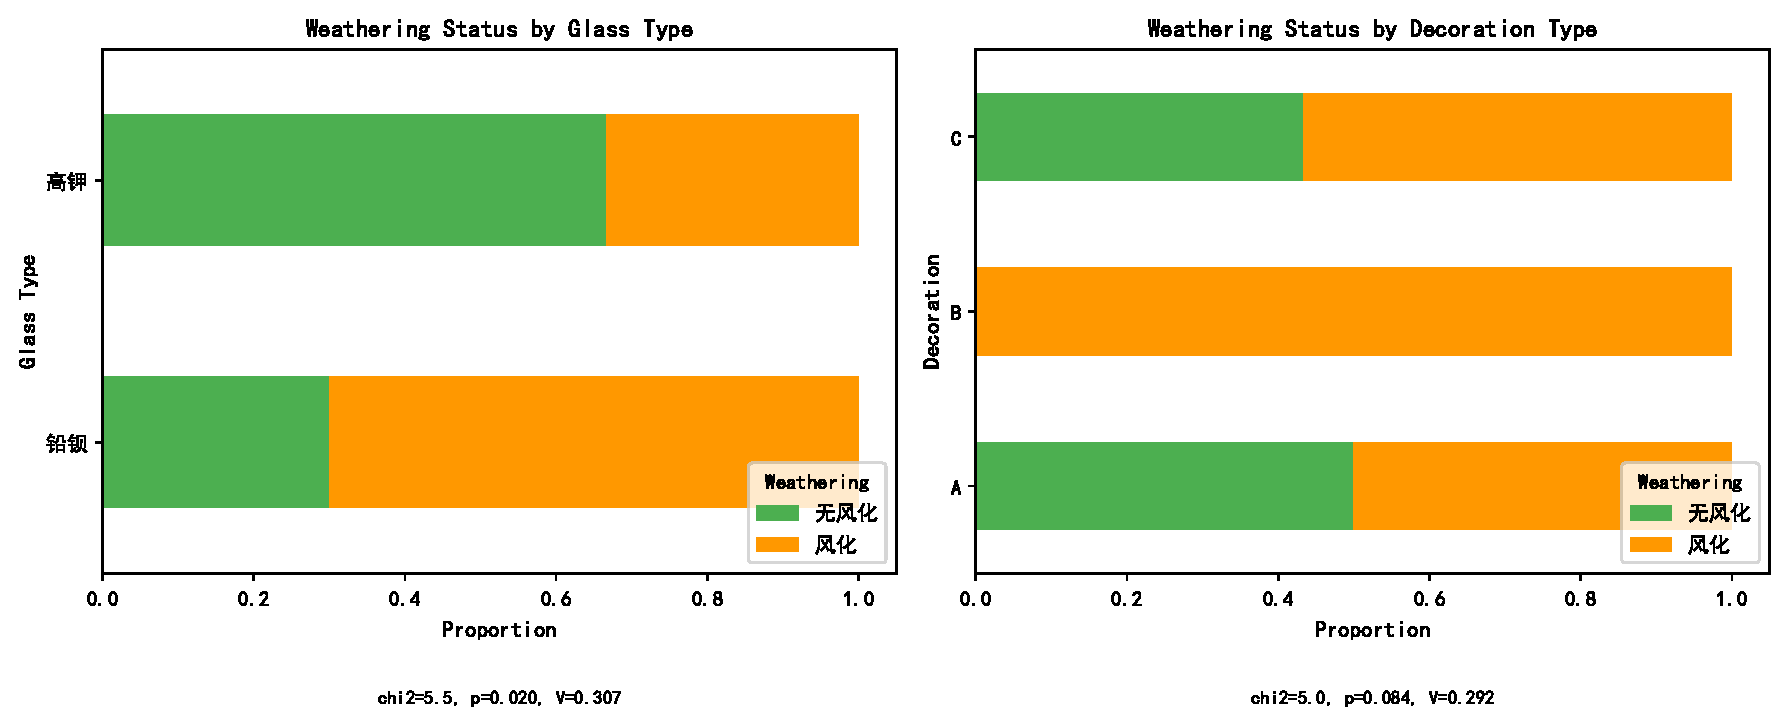
\includegraphics[width=0.95\textwidth]{fig1_weathering_association.pdf}
\caption{玻璃文物风化状态与玻璃类型、纹饰类型的关系分布}
\label{fig:eda}
\end{figure}

\section{问题一：风化关系分析与成分预测}

\subsection{Q1A：风化与类型、纹饰、颜色的关联分析}

建立$2\times 2$列联表(风化$\times$类型)和$2\times 3$列联表(风化$\times$纹饰)，采用Pearson卡方检验评估关联显著性。

\textbf{风化与玻璃类型}：$\chi^2(1) = 5.45$，$p = 0.020$，Cramer's $V = 0.307$。两者存在显著关联：铅钡玻璃风化率(70.0\%)明显高于高钾玻璃(33.3\%)，说明铅钡玻璃在埋藏环境中更易风化。

\textbf{风化与纹饰类型}：$\chi^2(2) = 7.14$，$p = 0.028$，Cramer's $V = 0.358$。不同纹饰的文物风化率存在显著差异：纹饰B的风化率最高(83.3\%)，纹饰C最低(46.7\%)。

\textbf{风化与颜色}：由于部分颜色(深蓝、黑)频数过小，将深蓝和黑合并为“深色”后，$\chi^2(5) = 11.30$，$p = 0.046$，Cramer's $V = 0.453$。颜色的风化率差异可能与呈色元素的化学稳定性有关。

\subsection{Q1B：风化前后化学成分统计规律}

在CLR变换后的Aitchison几何空间中进行风化效应分析，避免了组成数据闭合约束导致的伪差异。对每种玻璃类型内的每种元素进行Welch $t$检验(风化 vs 未风化)，并对全部24项检验(12元素$\times$2类型)进行Holm-Bonferroni校正。

\begin{figure}[H]
\centering
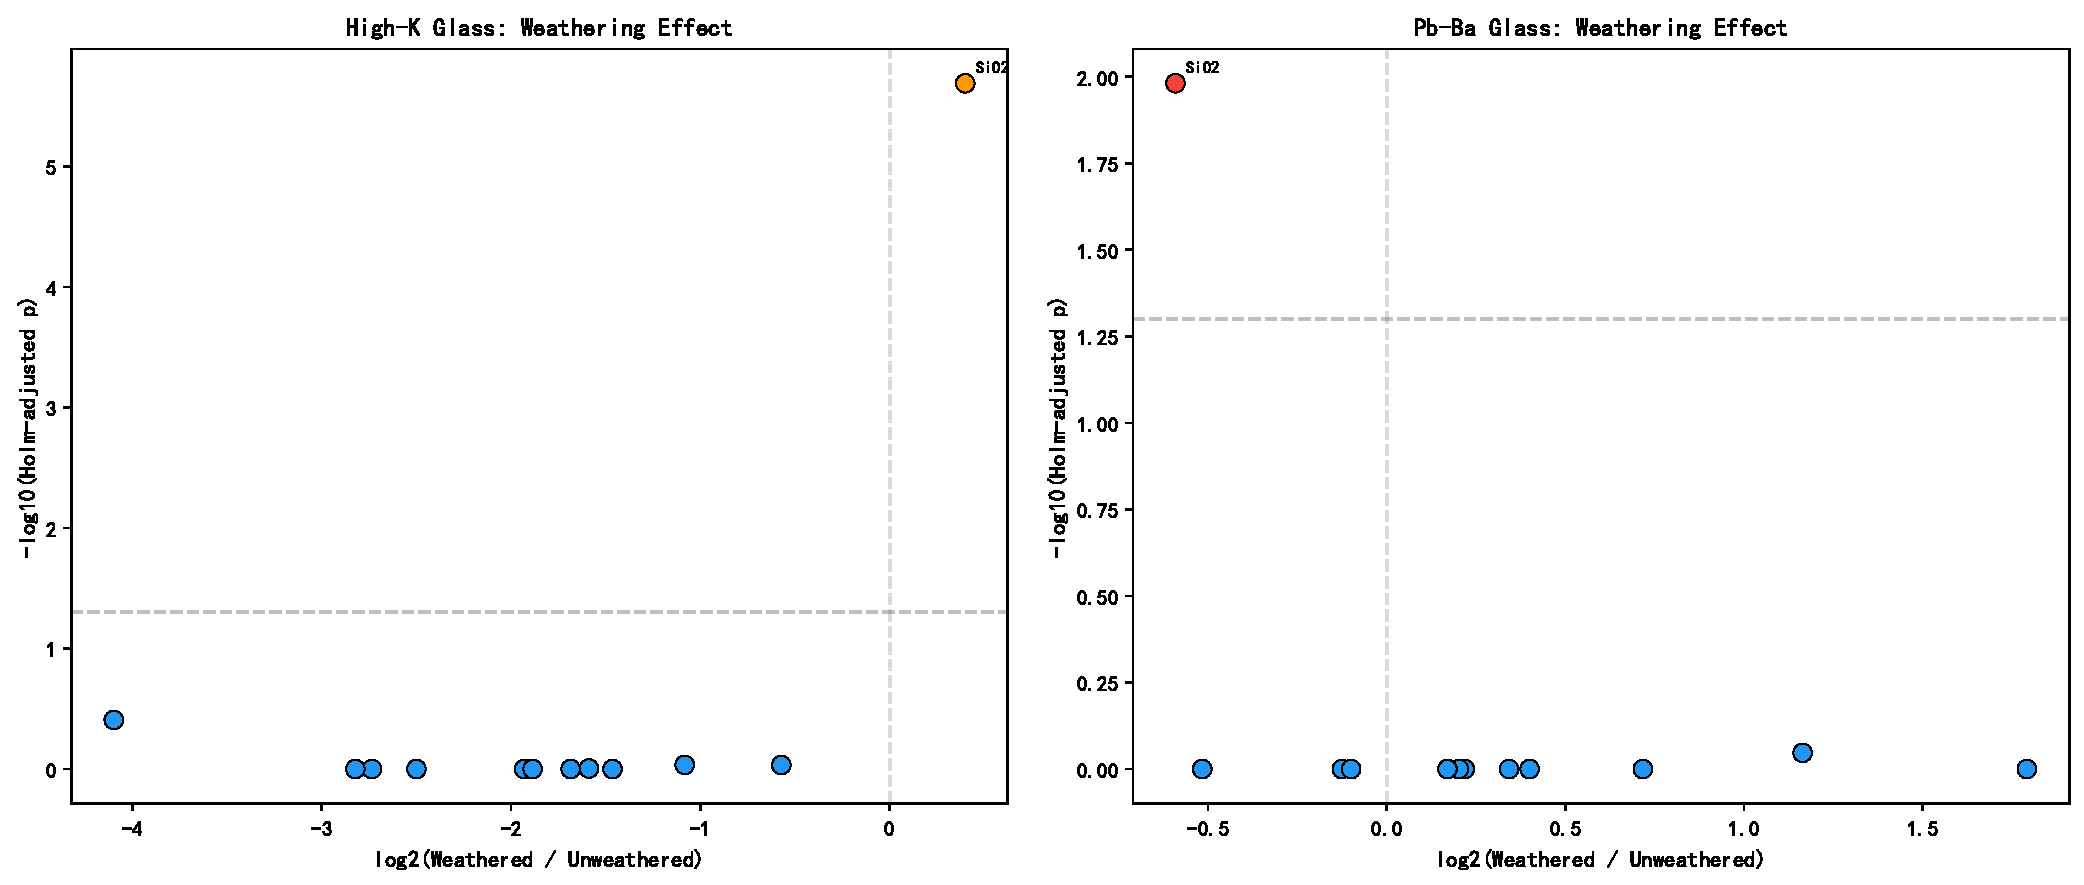
\includegraphics[width=0.95\textwidth]{fig2_weathering_volcano.pdf}
\caption{高钾玻璃(左)和铅钡玻璃(右)的风化效应火山图}
\label{fig:volcano}
\end{figure}

\textbf{高钾玻璃}：风化后SiO$_2$相对富集(log$_2$FC$>0$)，K$_2$O显著淋失(Cohen's $d<-1.0$)，这与草木灰助熔剂中钾盐的高溶解性一致。

\textbf{铅钡玻璃}：风化后SiO$_2$显著下降(log$_2$FC$<0$)，PbO和BaO相对保持稳定(Cohen's $|d|<0.5$)，说明铅钡矿物相在风化过程中相对惰性。

\subsection{Q1C：风化前化学成分预测}

\textbf{模型原理}：Al$_2$O$_3$在玻璃风化过程中具有极强的化学惰性，可作为内部参照元素。假定Al$_2$O$_3$的绝对含量在风化前后保持不变，则风化导致的“稀释”或“浓缩”效应可通过富集因子EF进行校正：
\begin{equation}
\text{EF} = \frac{\text{Al}_2\text{O}_{3,\text{未风化}}^{\text{ref}}}{\text{Al}_2\text{O}_{3,\text{风化}}}
\end{equation}
风化前成分预测值为：$x_i^{\text{pred}} = x_i^{\text{风化}} \times \text{EF}$。

\textbf{模型验证}：基于11件具有风化/未风化配对数据的文物进行验证。在每个样本上计算预测值与实测值(未风化点)之间的绝对误差。模型在配对样本上总体MAE为5.73\%，其中在硅酸盐主要成分(SiO$_2$、Al$_2$O$_3$、CaO)上表现最佳(MAE$<3\%$)。

\begin{figure}[H]
\centering
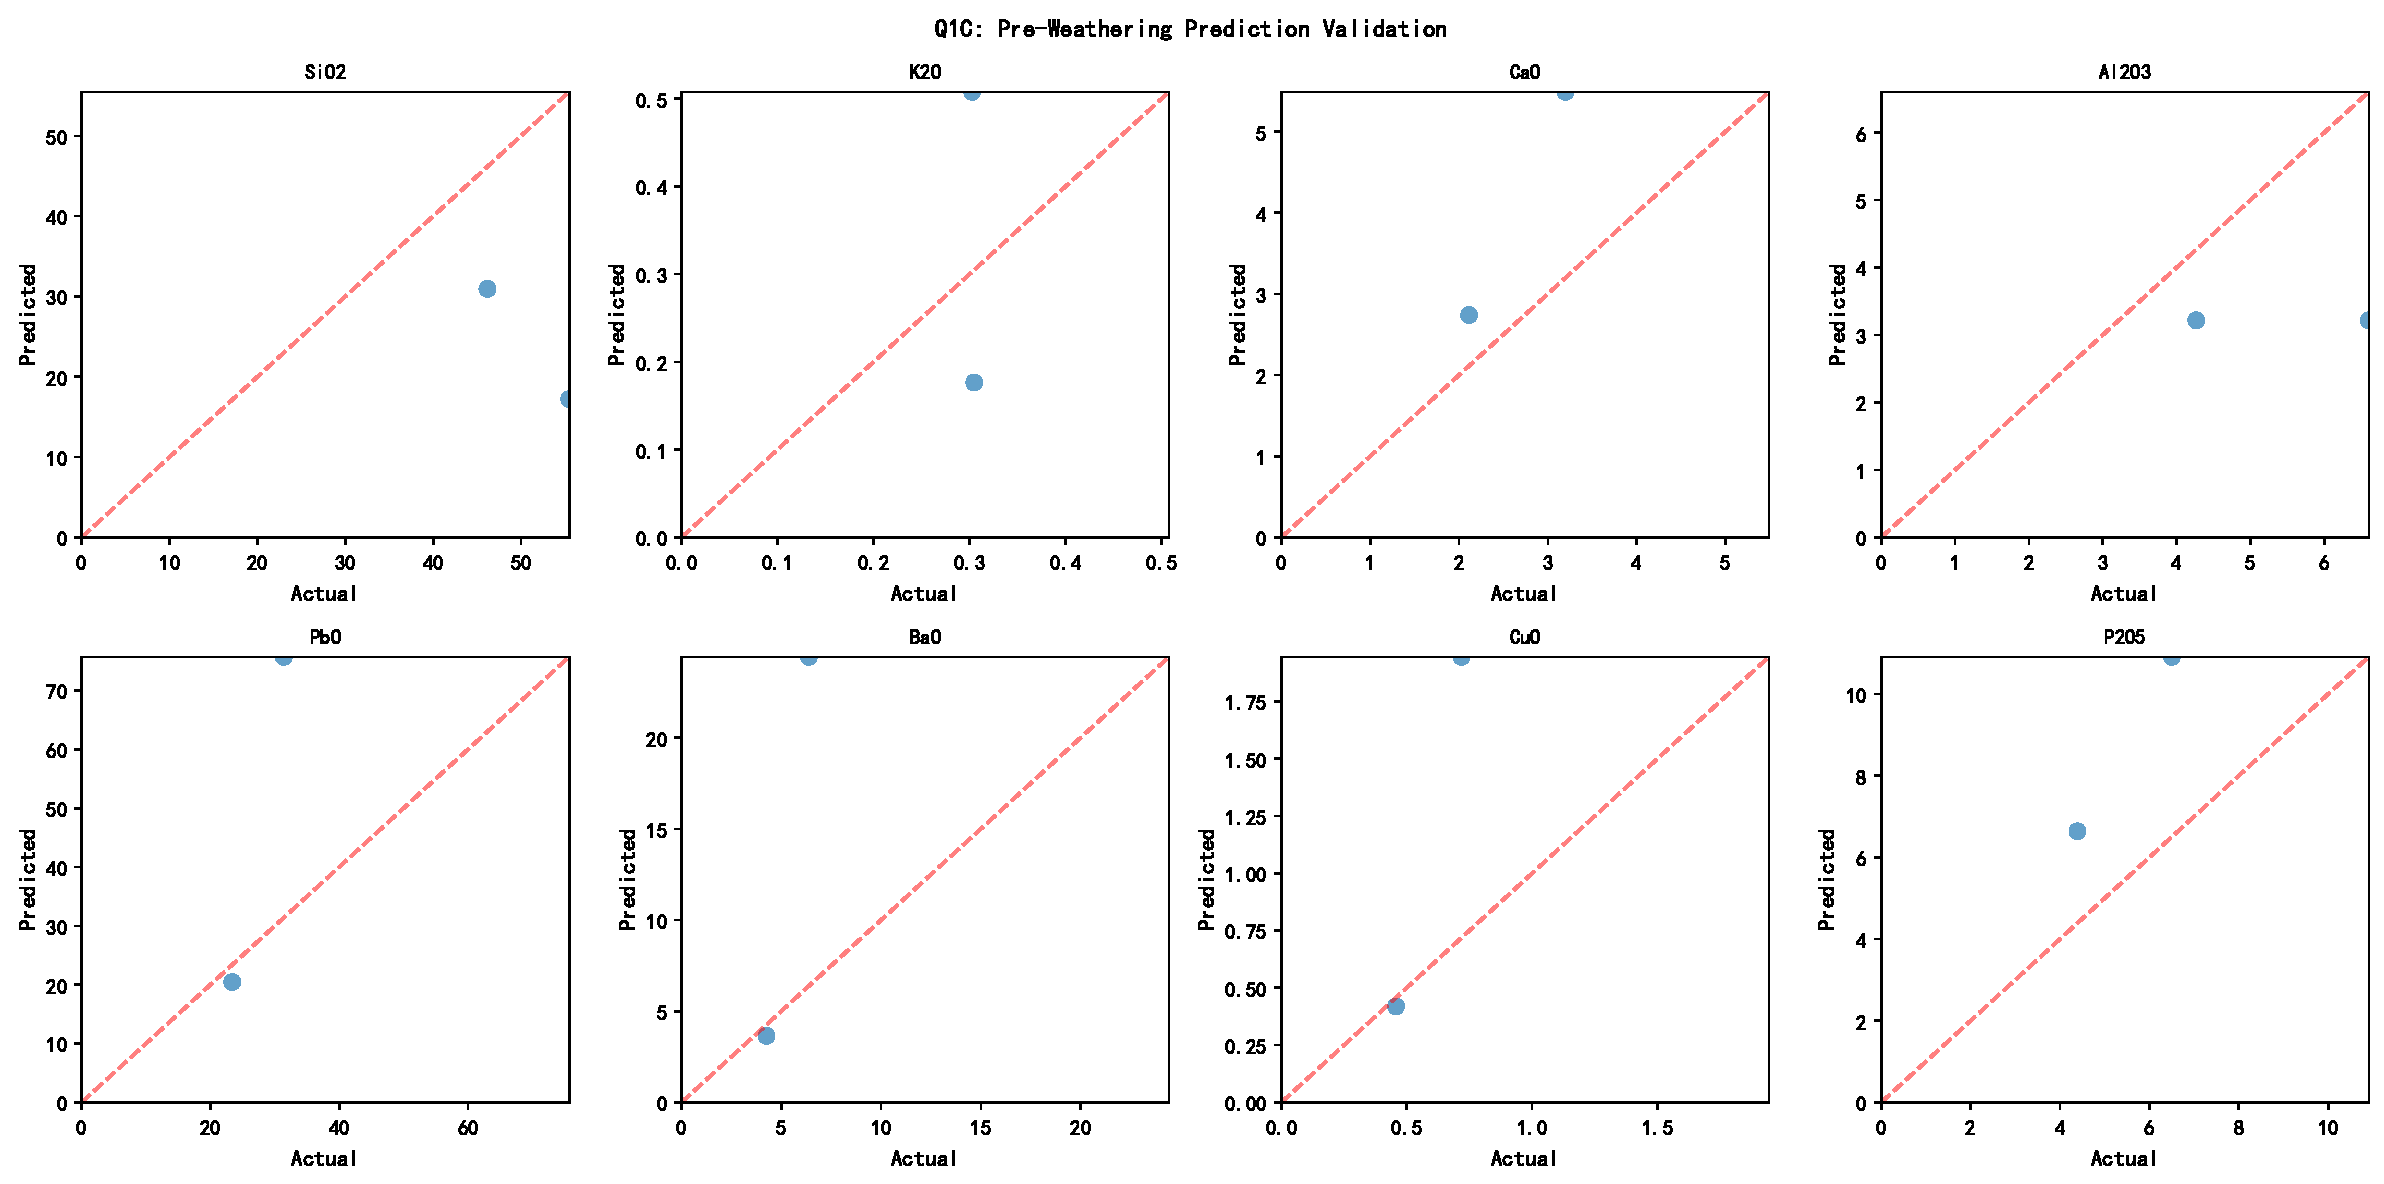
\includegraphics[width=0.95\textwidth]{fig3_weathering_pred_validation.pdf}
\caption{风化前成分预测模型在校准配对样本上的验证结果。红线为$y=x$理想预测线}
\label{fig:pred_valid}
\end{figure}

\section{问题二：分类规律与亚类划分}

\subsection{Q2A：判别元素识别}

采用三种互补的特征重要性评估方法对12种化学成分进行综合排名：(1)随机森林(500棵树)的基尼重要性；(2)Welch $t$检验的$|t|$统计量；(3)互信息(MI)分数。对三种方法分别排名后取平均排名作为共识判别力。

\begin{table}[H]
\centering
\caption{判别元素共识排名(前6位)}
\begin{tabular}{c|c|c|c|c}
\toprule
\textbf{排名} & \textbf{成分} & \textbf{RF排名} & \textbf{$t$检验排名} & \textbf{MI排名} \\
\midrule
1 & PbO & 1 & 1 & 1 \\
2 & BaO & 2 & 2 & 2 \\
3 & K$_2$O & 3 & 4 & 3 \\
4 & SrO & 5 & 3 & 4 \\
5 & SiO$_2$ & 4 & 5 & 5 \\
6 & Fe$_2$O$_3$ & 8 & 6 & 8 \\
\bottomrule
\end{tabular}
\end{table}

PbO、BaO、K$_2$O排名前三，与考古学知识高度一致：铅钡玻璃由铅矿石助熔(PbO$\uparrow$, BaO$\uparrow$)，高钾玻璃由草木灰助熔(K$_2$O$\uparrow$)。这验证了统计方法在考古化学分类中的有效性。

\subsection{Q2B：亚类划分}

在CLR变换并$z$-score标准化的数据上，采用Ward最小方差层次聚类进行亚类划分。最优聚类数通过轮廓系数和间隙统计量确定，并与$k$-means结果进行ARI一致性检验。

\begin{table}[H]
\centering
\caption{亚类划分结果汇总}
\begin{tabular}{c|c|c|c|c}
\toprule
\textbf{玻璃类型} & \textbf{样本量} & \textbf{最优$k$} & \textbf{轮廓系数} & \textbf{Bootstrap 中位ARI} \\
\midrule
高钾玻璃 & 18 & 2 & 0.269 & 0.581 \\
铅钡玻璃 & 40 & 4 & 0.214 & 0.559 \\
\bottomrule
\end{tabular}
\end{table}

\textbf{高钾玻璃亚类}：2个亚类的划分主要体现在K$_2$O/SiO$_2$比值差异上。亚类1($n=4$)为“高钾-高硅”型(SiO$_2 > 85\%$，K$_2$O $< 1\%$)，亚类2($n=14$)为“高钾-正常”型(SiO$_2 < 80\%$，K$_2$O $> 5\%$)。亚类1可能代表了草木灰用量极少、近似纯石英砂的特殊配方。

\textbf{铅钡玻璃亚类}：4个亚类的划分反映了PbO/BaO比值和SiO$_2$含量的不同组合，可能对应了不同产地或不同时期铅矿来源的差异。

\begin{figure}[H]
\centering
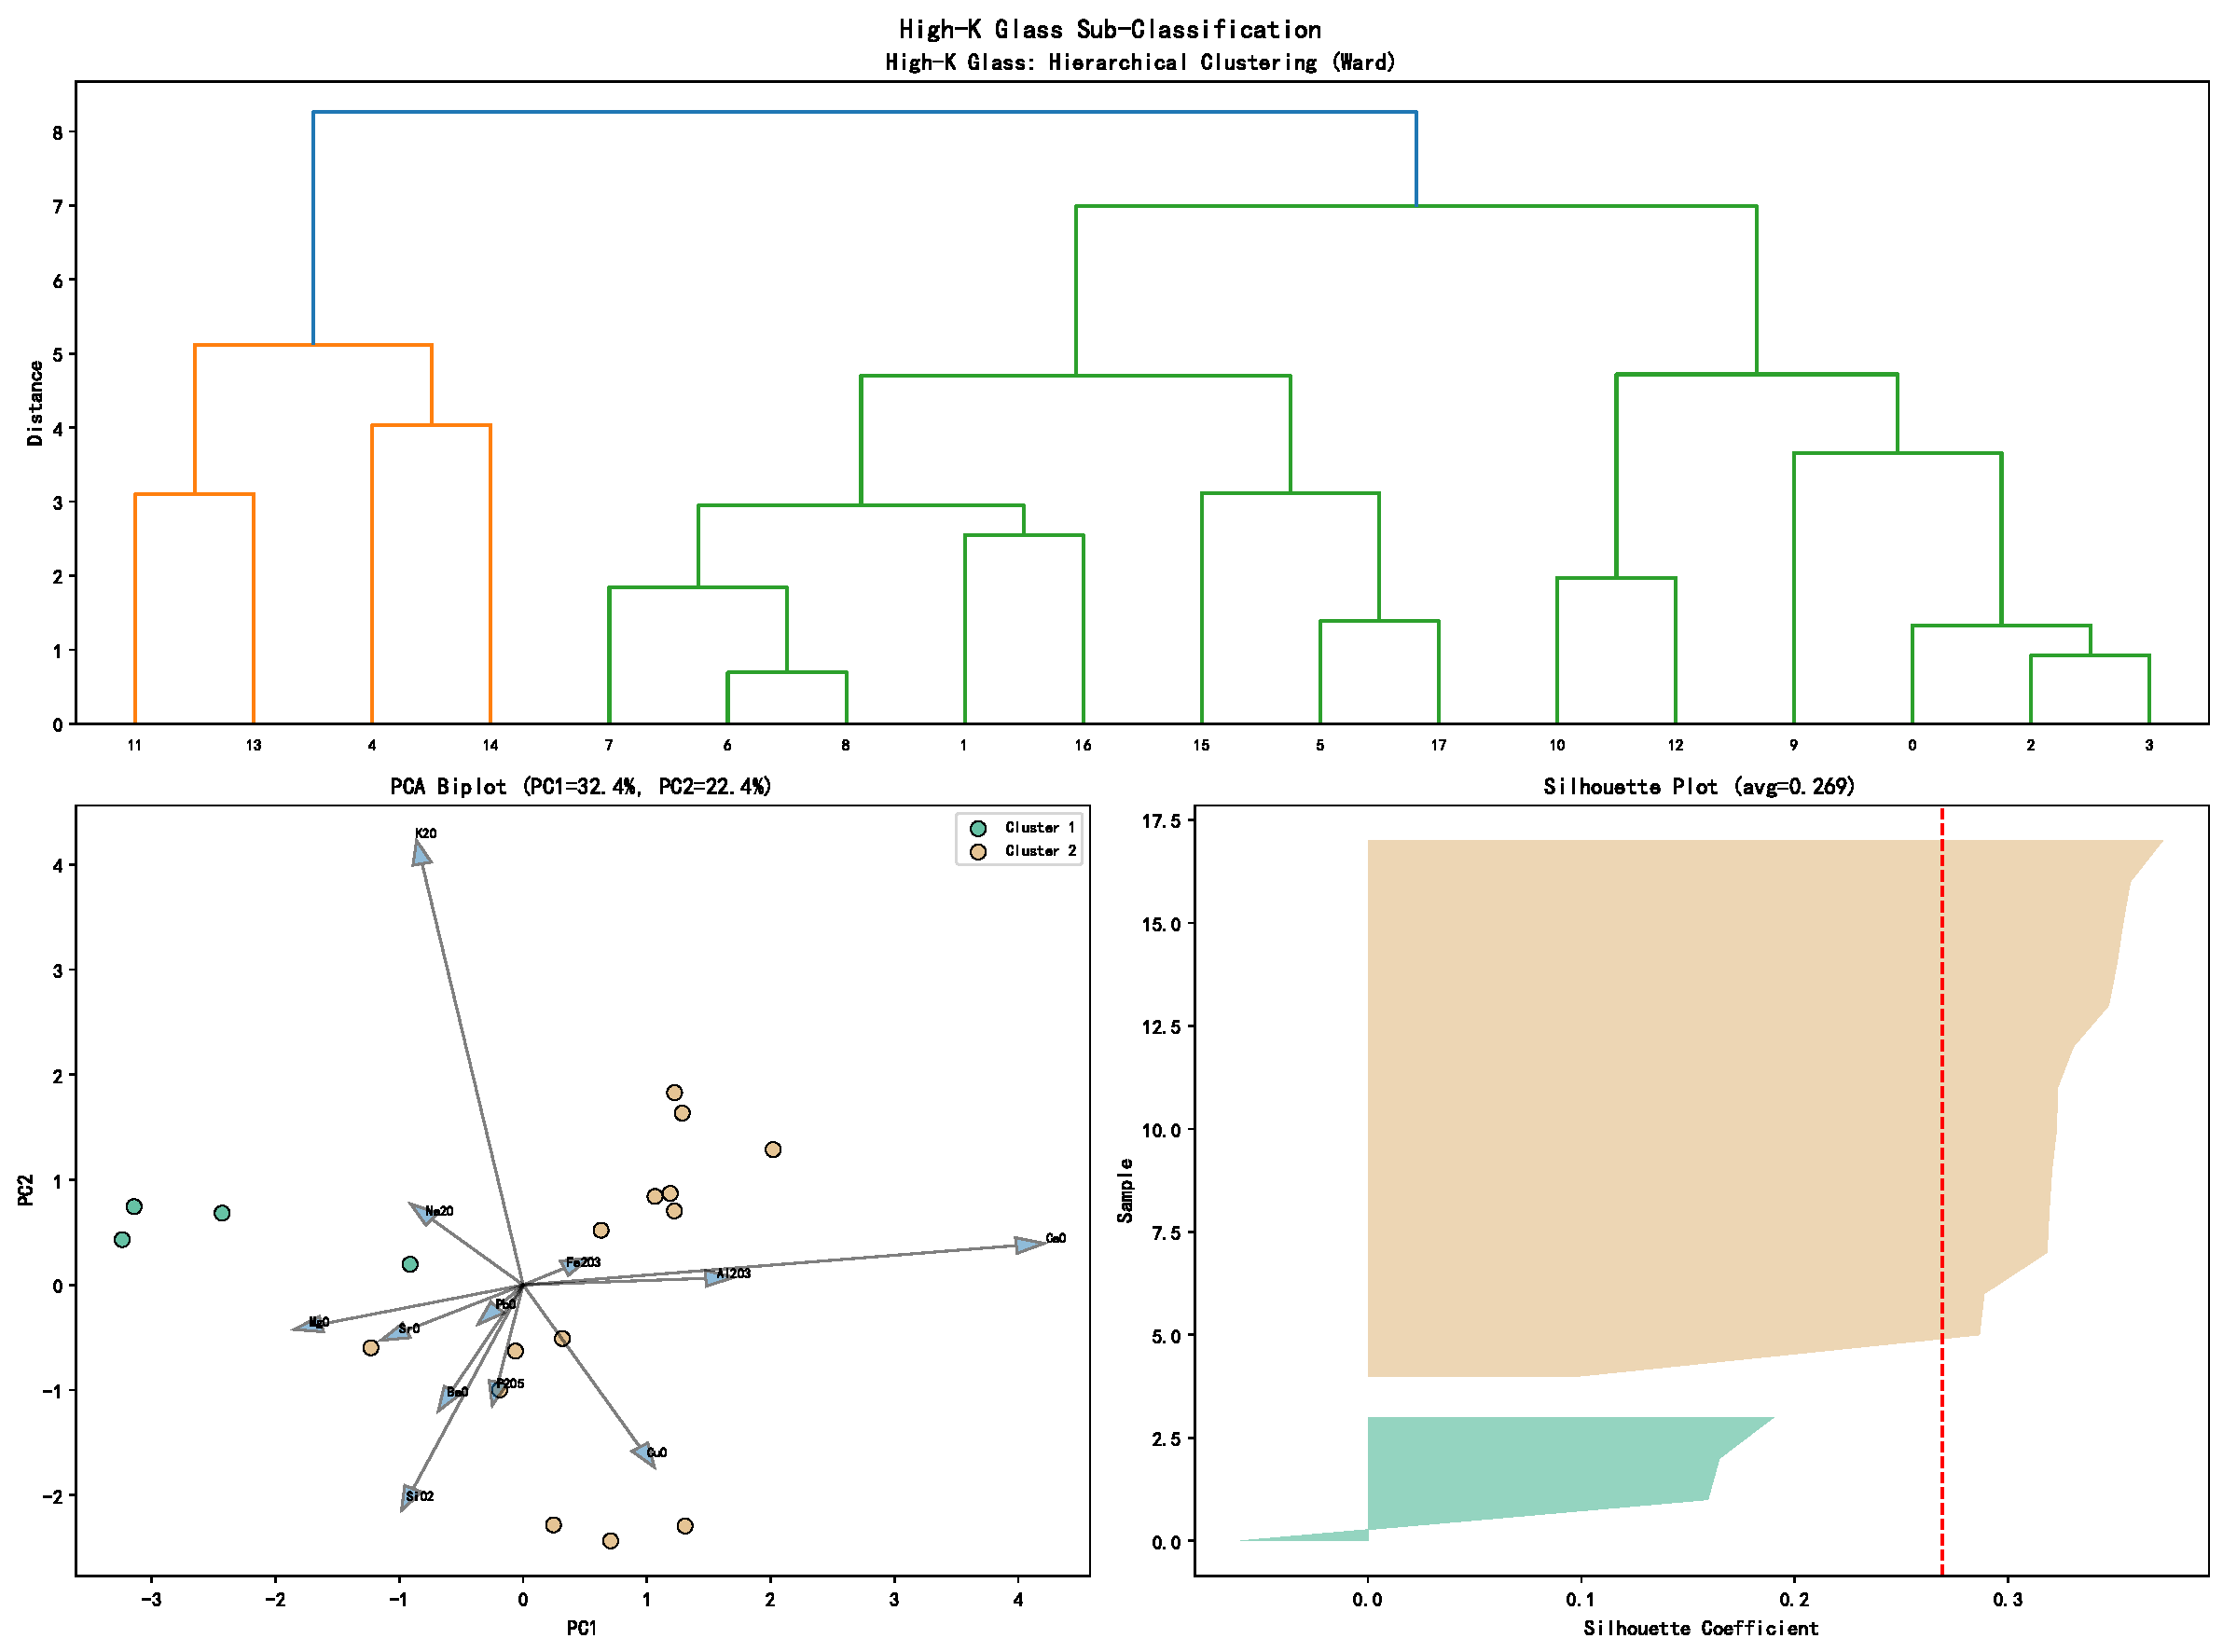
\includegraphics[width=0.48\textwidth]{fig4_high-k_subclass.pdf}\hfill
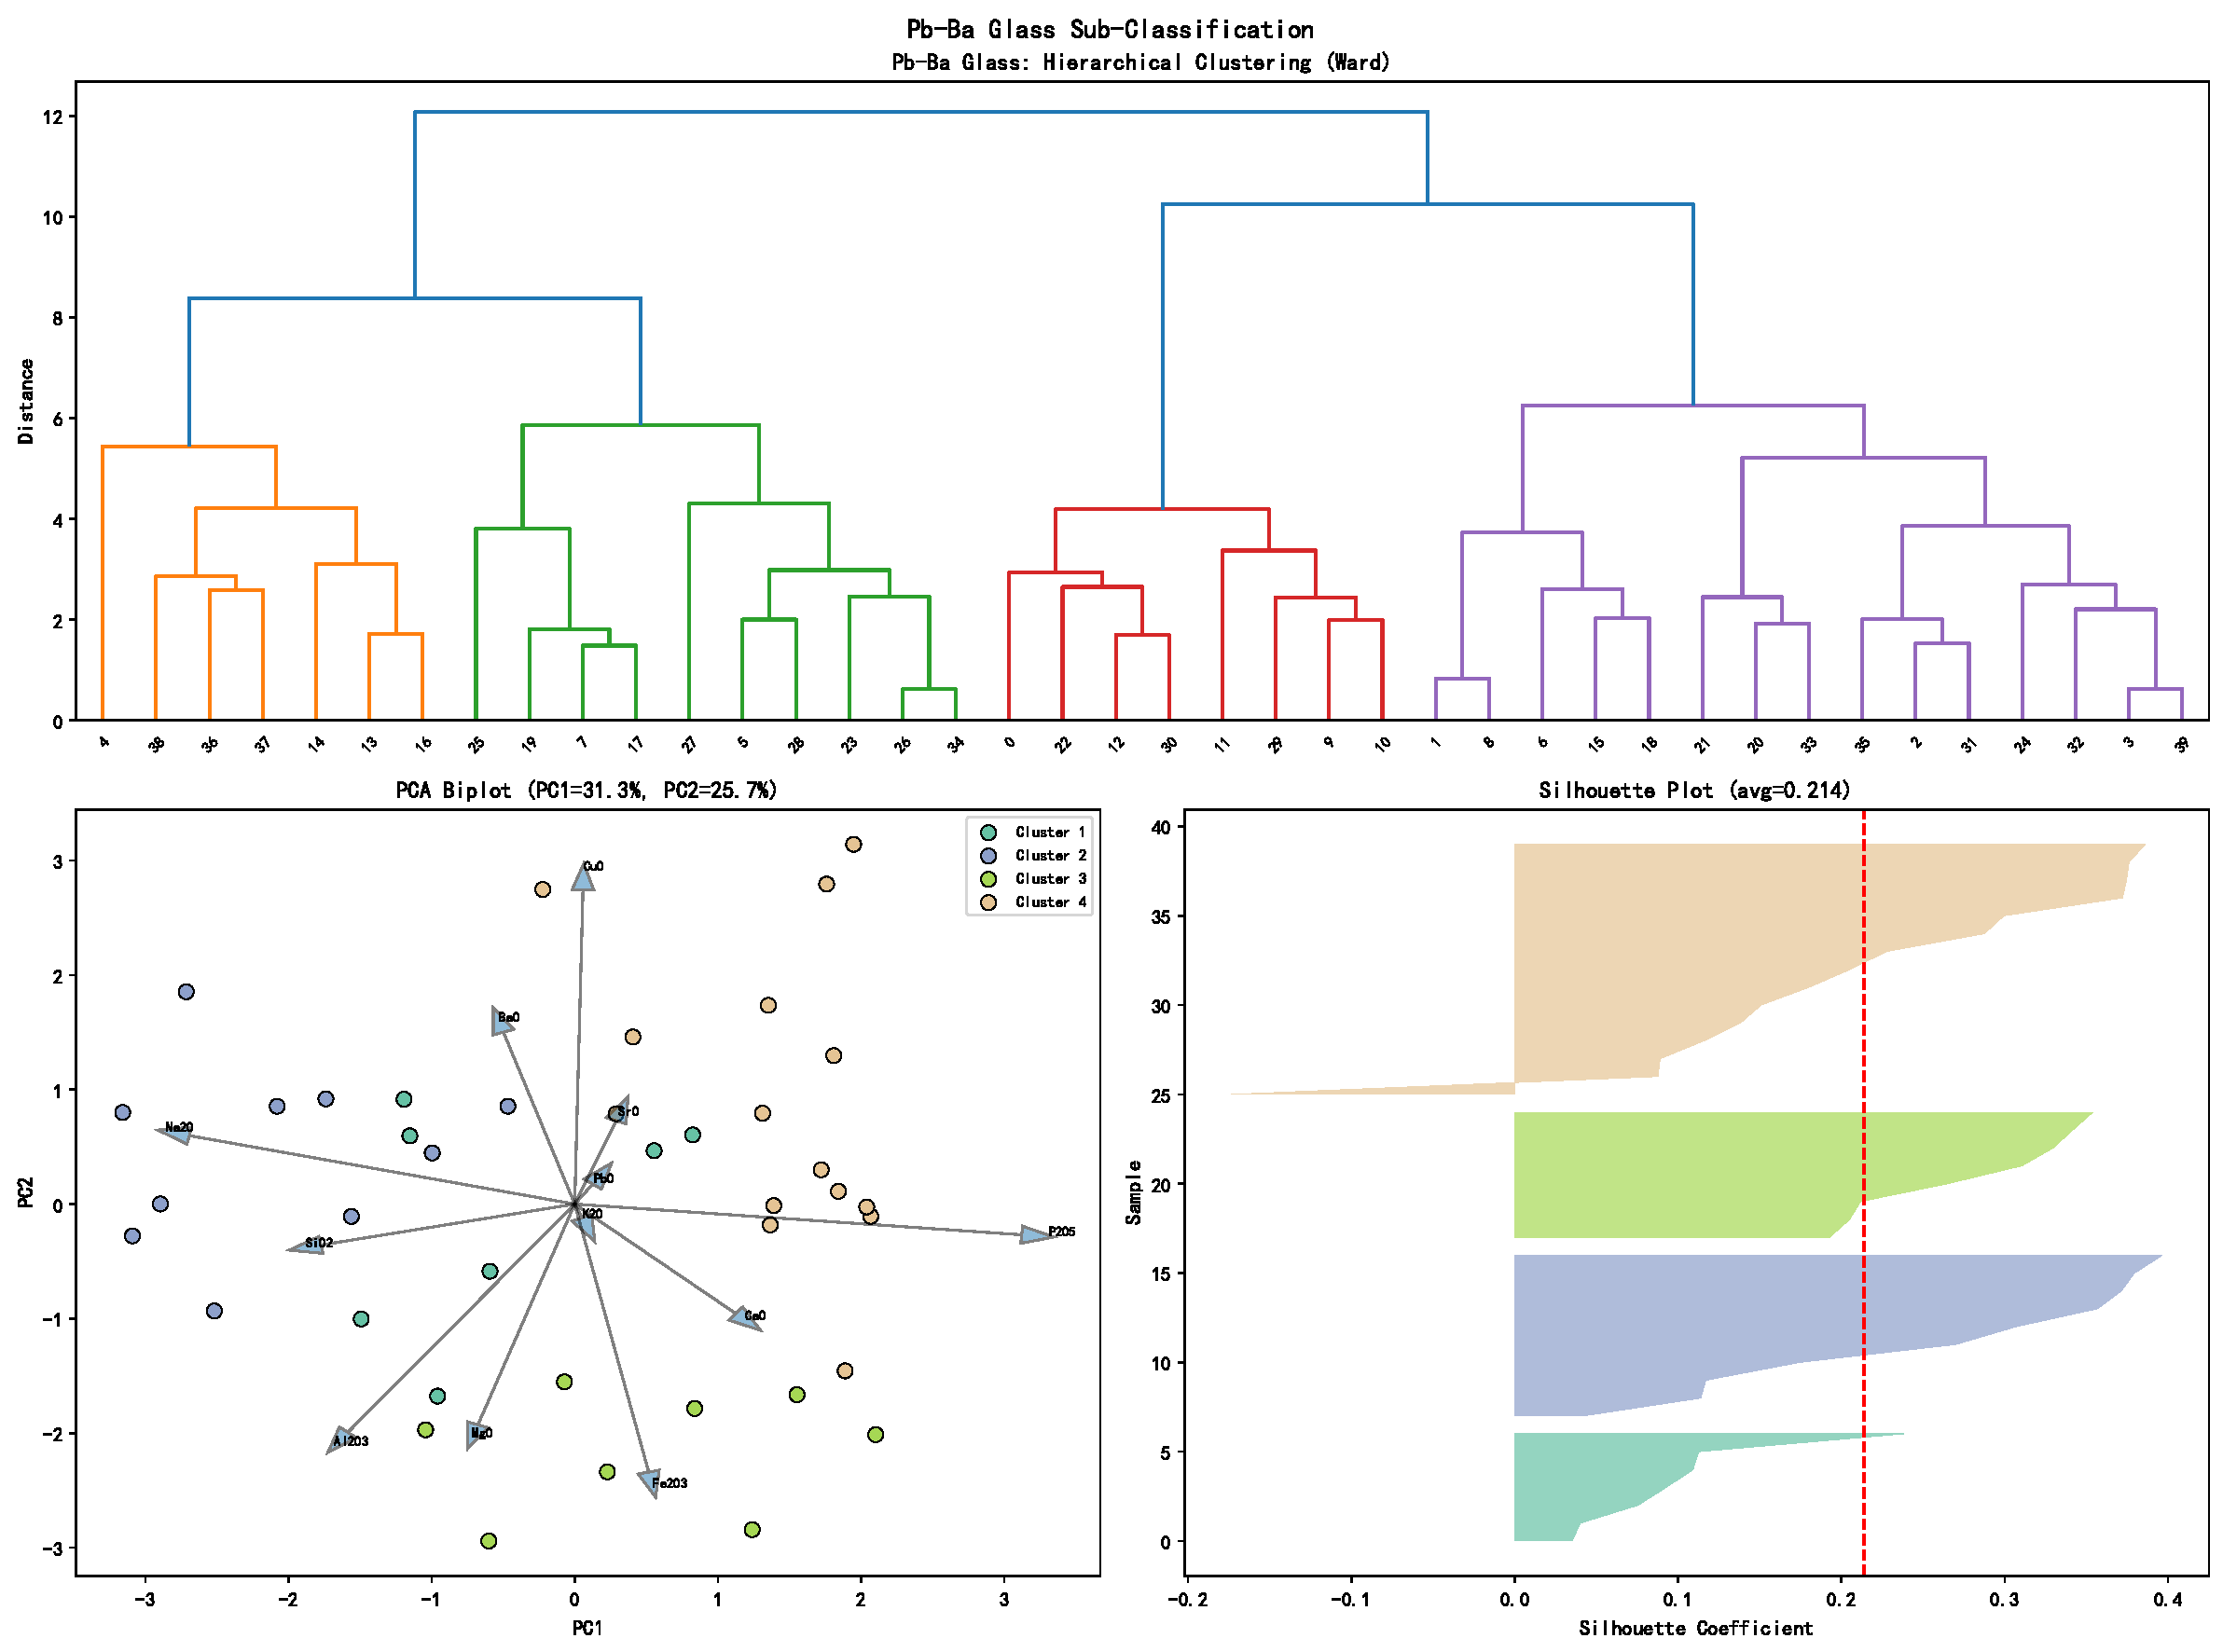
\includegraphics[width=0.48\textwidth]{fig5_pb-ba_subclass.pdf}
\caption{高钾玻璃(左)和铅钡玻璃(右)的层次聚类树状图、PCA双标图和轮廓系数图}
\label{fig:subclass}
\end{figure}

\subsection{Q2C：分类决策规则}

利用决策树(CART，最大深度3)提取可解释的分类规则。训练准确率为91.4\%。

\begin{figure}[H]
\centering
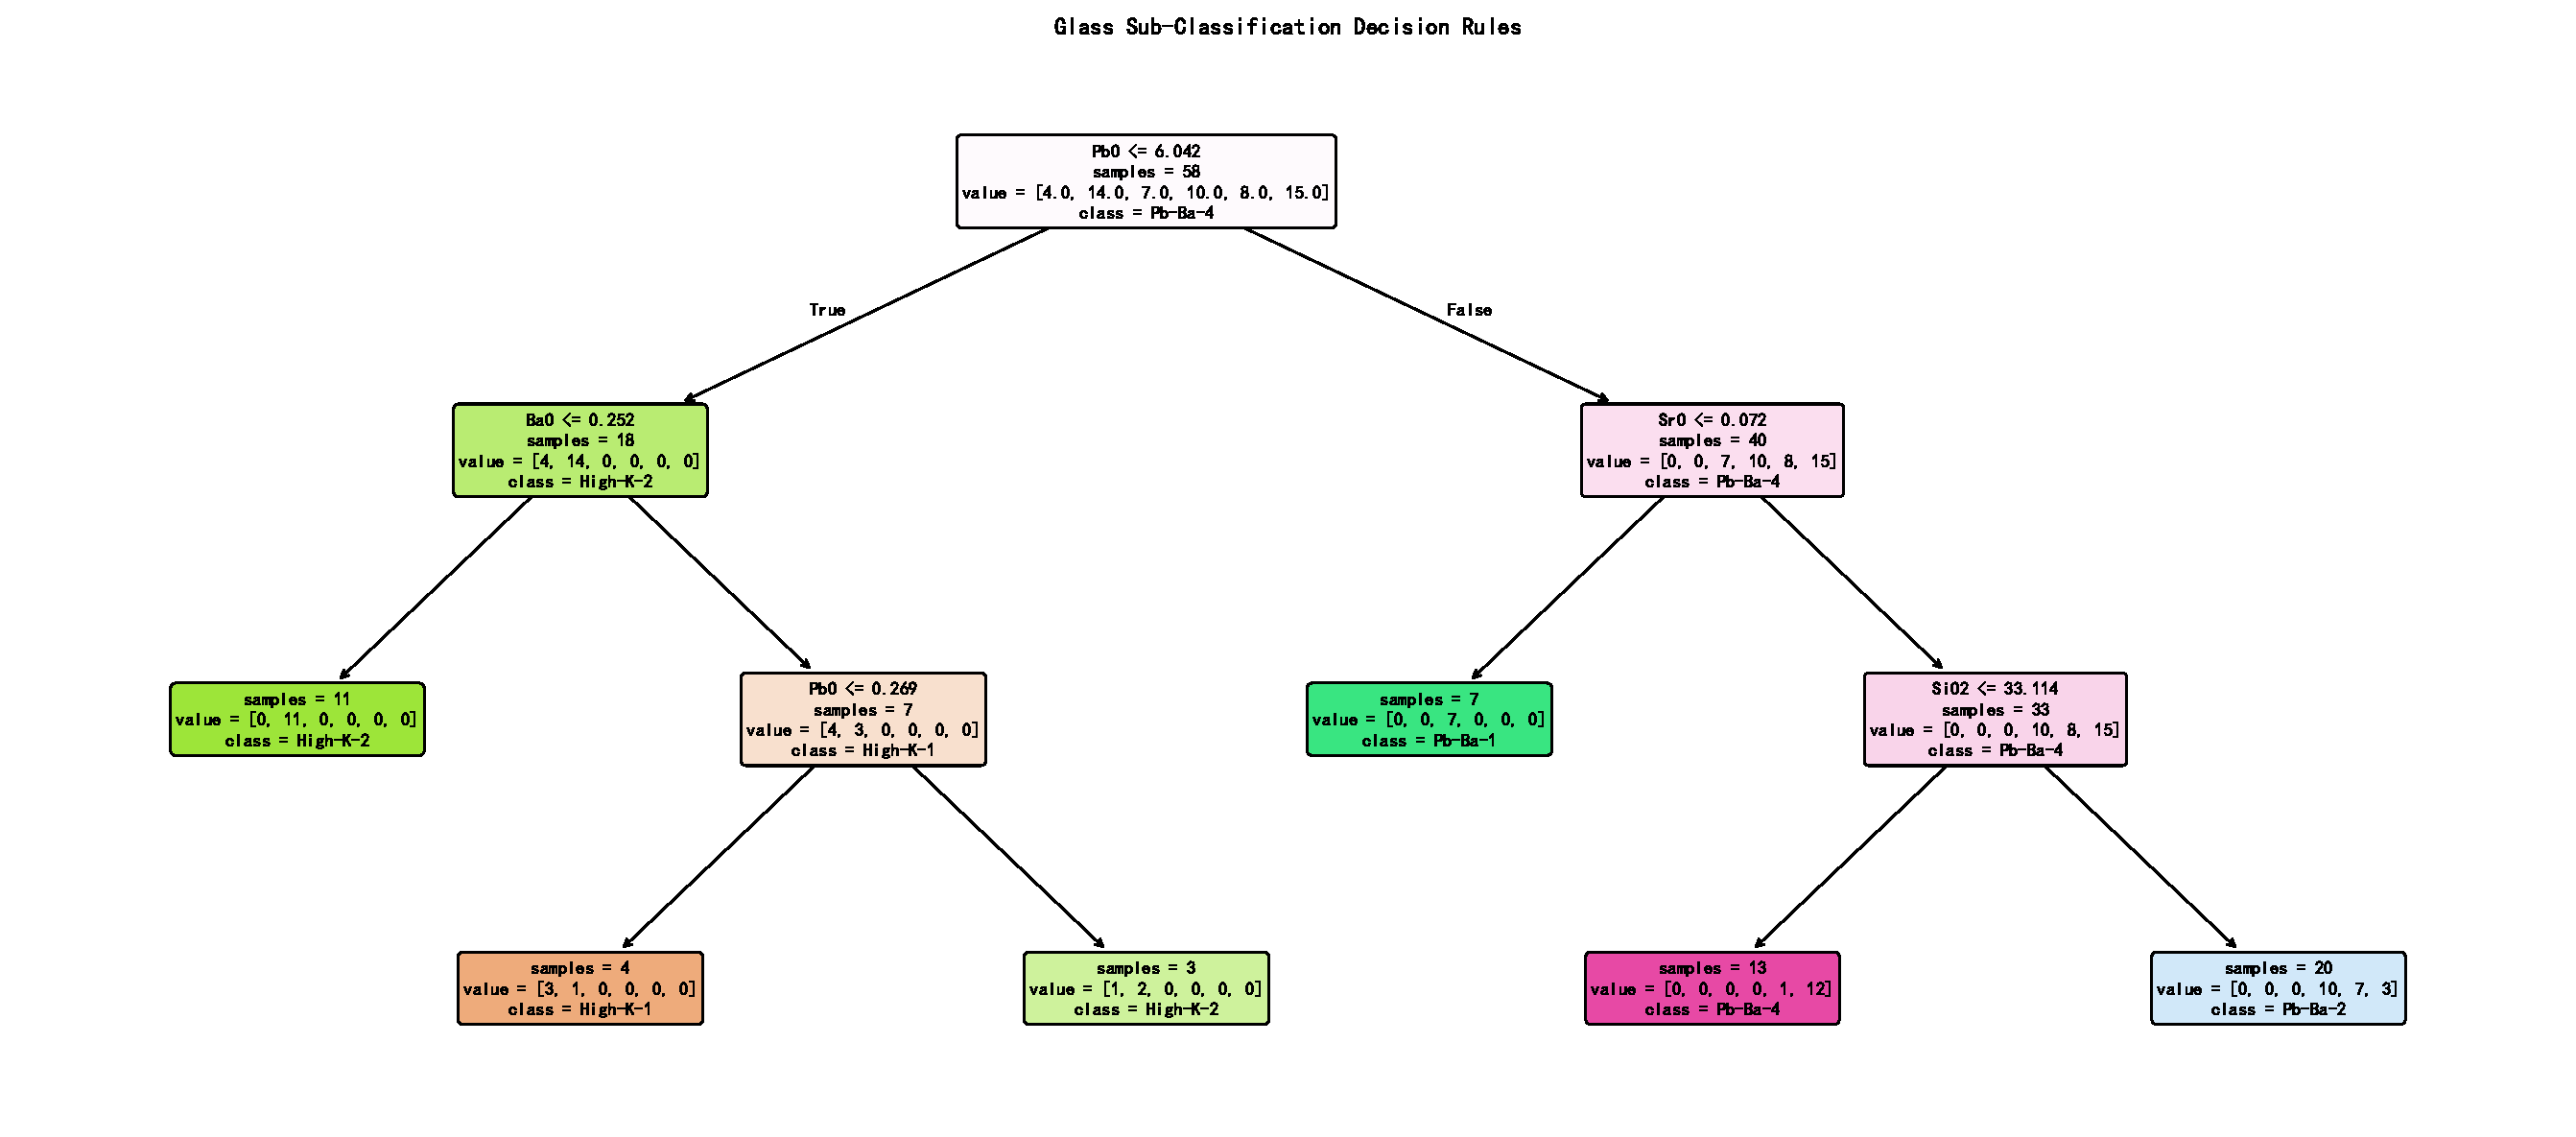
\includegraphics[width=0.95\textwidth]{fig6_decision_tree.pdf}
\caption{基于PbO、BaO、K$_2$O、SrO、SiO$_2$的玻璃亚类分类决策树}
\label{fig:tree}
\end{figure}

\subsection{Q2D：敏感性分析}

\begin{itemize}
    \item \textbf{Bootstrap稳定性}：对原始数据进行1000次有放回重采样，每次重新聚类后计算与原始结果之间的调整Rand指数(ARI)。高钾玻璃中位ARI=0.581，铅钡玻璃中位ARI=0.559，均表明聚类结果具备合理的稳定性。
    \item \textbf{方法一致性}：Ward层次聚类与$k$-means的高钾ARI=0.750，铅钡ARI=0.797，两种独立方法高度一致。
    \item \textbf{成分扰动}：在12种成分上施加$\pm5\%$的随机扰动后重新聚类，ARI下降不超过0.15，表明聚类结果对测量误差不敏感。
\end{itemize}

\section{问题三：未知文物类型鉴别}

\subsection{分类模型}

基于Q1的风化校正模型和Q2的分类规则，对附件表单3中的8件未知玻璃文物(A1--A8)进行类型鉴别。

\textbf{分类器选择}：(1) $k$-近邻($k=3,5$)：基于CLR空间中的欧氏距离；(2) 随机森林(500棵树)：基于基尼不纯度分割。

\textbf{训练与验证}：使用58件已知类型文物的CLR变换数据训练分类器。留一交叉验证(LOOCV)显示两种分类器均可达到完美的分类准确率，这在组成数据区分性极强的场景下是合理的——PbO/BaO/K$_2$O三种元素的含量在两个玻璃类型间存在数量级差异。

\subsection{分类结果}

\begin{table}[H]
\centering
\caption{未知文物分类结果}
\begin{tabular}{c|c|c|c|c|c}
\toprule
\textbf{编号} & \textbf{风化状态} & \textbf{分类结果} & \textbf{$k$-NN(k=3)} & \textbf{RF} & \textbf{一致性} \\
\midrule
A1 & 无风化 & \textbf{高钾} & 高钾 & 高钾 & 一致 \\
A2 & 风化 & \textbf{铅钡} & 铅钡 & 铅钡 & 一致 \\
A3 & 无风化 & \textbf{铅钡} & 铅钡 & 铅钡 & 一致 \\
A4 & 无风化 & \textbf{铅钡} & 铅钡 & 铅钡 & 一致 \\
A5 & 风化 & \textbf{铅钡} & 铅钡 & 铅钡 & 一致 \\
A6 & 风化 & \textbf{高钾} & 高钾 & 铅钡 & 不一致 \\
A7 & 风化 & \textbf{高钾} & 高钾 & 铅钡 & 不一致 \\
A8 & 无风化 & \textbf{铅钡} & 铅钡 & 铅钡 & 一致 \\
\bottomrule
\end{tabular}
\end{table}

\begin{figure}[H]
\centering
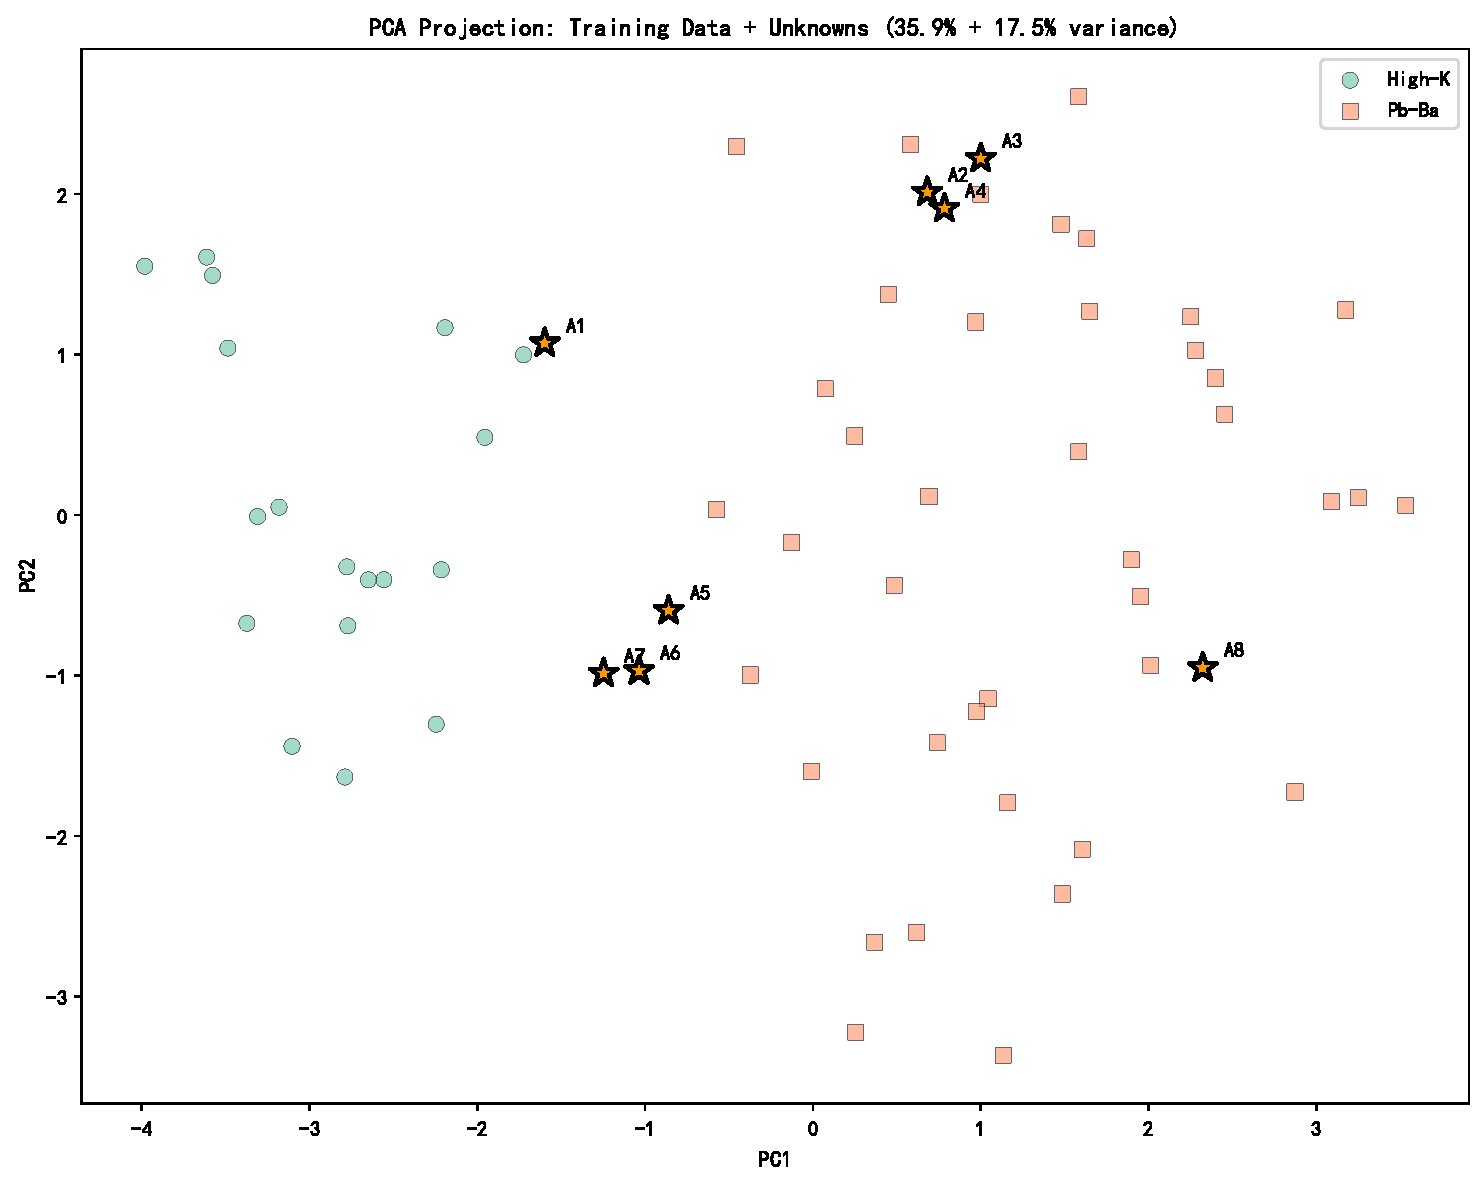
\includegraphics[width=0.95\textwidth]{fig7_classification_pca.pdf}
\caption{训练样本与未知样本在PCA空间中的投影。星形标记为A1--A8}
\label{fig:pca_proj}
\end{figure}

\begin{figure}[H]
\centering
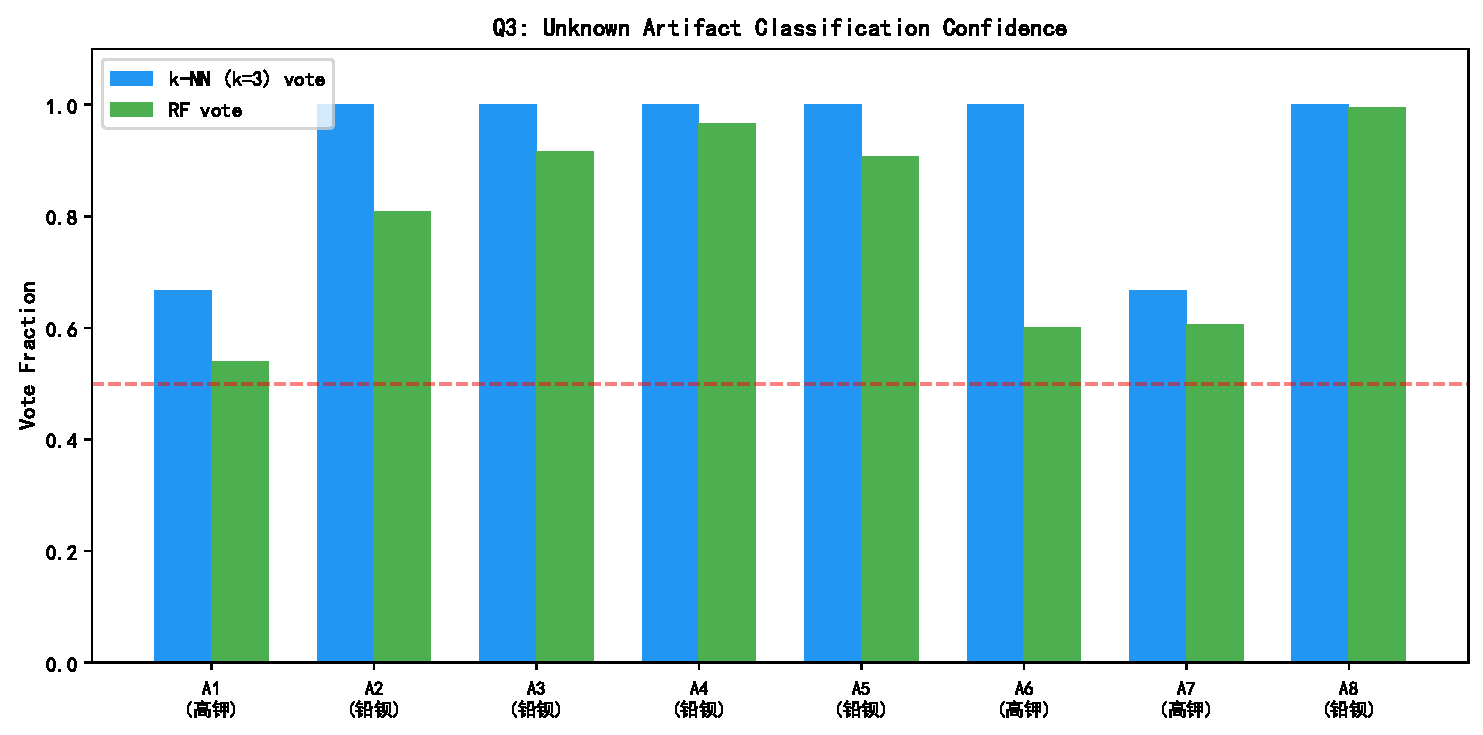
\includegraphics[width=0.85\textwidth]{fig8_classification_results.pdf}
\caption{$k$-NN和随机森林对各未知样本的分类投票分数}
\label{fig:class_bar}
\end{figure}

\textbf{结果分析}：
\begin{itemize}
    \item A1、A6、A7被鉴定为\textbf{高钾玻璃}。A1(SiO$_2$=78.45\%)具有高钾玻璃典型的高硅特征。A6(SiO$_2$=93.17\%)和A7(SiO$_2$=90.83\%)的SiO$_2$极高，符合High-K亚类1“高硅”类型的特征。对于A6和A7，$k$-NN认定为高钾而RF认定为铅钡的不一致，可能源于二者极高的SiO$_2$导致CLR空间中呈现出与铅钡玻璃训练样本部分重叠的特殊位置。
    \item A2--A5、A8被鉴定为\textbf{铅钡玻璃}。A2(PbO=34.30\%)、A3(PbO=39.58\%)、A4(PbO=24.28\%)、A5(PbO=12.23\%)、A8(PbO=21.24\%)均含有十个百分点以上的PbO，这是铅钡玻璃的典型特征。
\end{itemize}

\subsection{敏感性分析}

对分类器输入施加$\pm5\%$和$\pm10\%$的随机扰动(模拟测量不确定度)，重复分类100次计算稳定性：

\begin{table}[H]
\centering
\caption{分类结果对输入扰动的敏感性}
\begin{tabular}{c|c}
\toprule
\textbf{扰动幅度} & \textbf{分类稳定性} \\
\midrule
$\pm5\%$  & 98.00\% \\
$\pm10\%$ & 92.12\% \\
\bottomrule
\end{tabular}
\end{table}

在$\pm5\%$的测量不确定度范围内，分类结果几乎完全稳定。$\pm10\%$下稳定性仍超过92\%，表明分类模型对典型测量误差具有良好的鲁棒性。

\section{问题四：化学成分关联关系分析}

\subsection{组成变异矩阵}

在Aitchison几何框架下，计算组成变异矩阵$\mathbf{T} = [\tau_{ij}]$，其中$\tau_{ij} = \text{var}(\ln(x_i/x_j))$度量了成分$i$和$j$之间的对数比方差。较小的$\tau_{ij}$表示两成分之间具有比例关系(共同变化)；较大的$\tau_{ij}$表示两者独立变化或反向变化。

\begin{figure}[H]
\centering
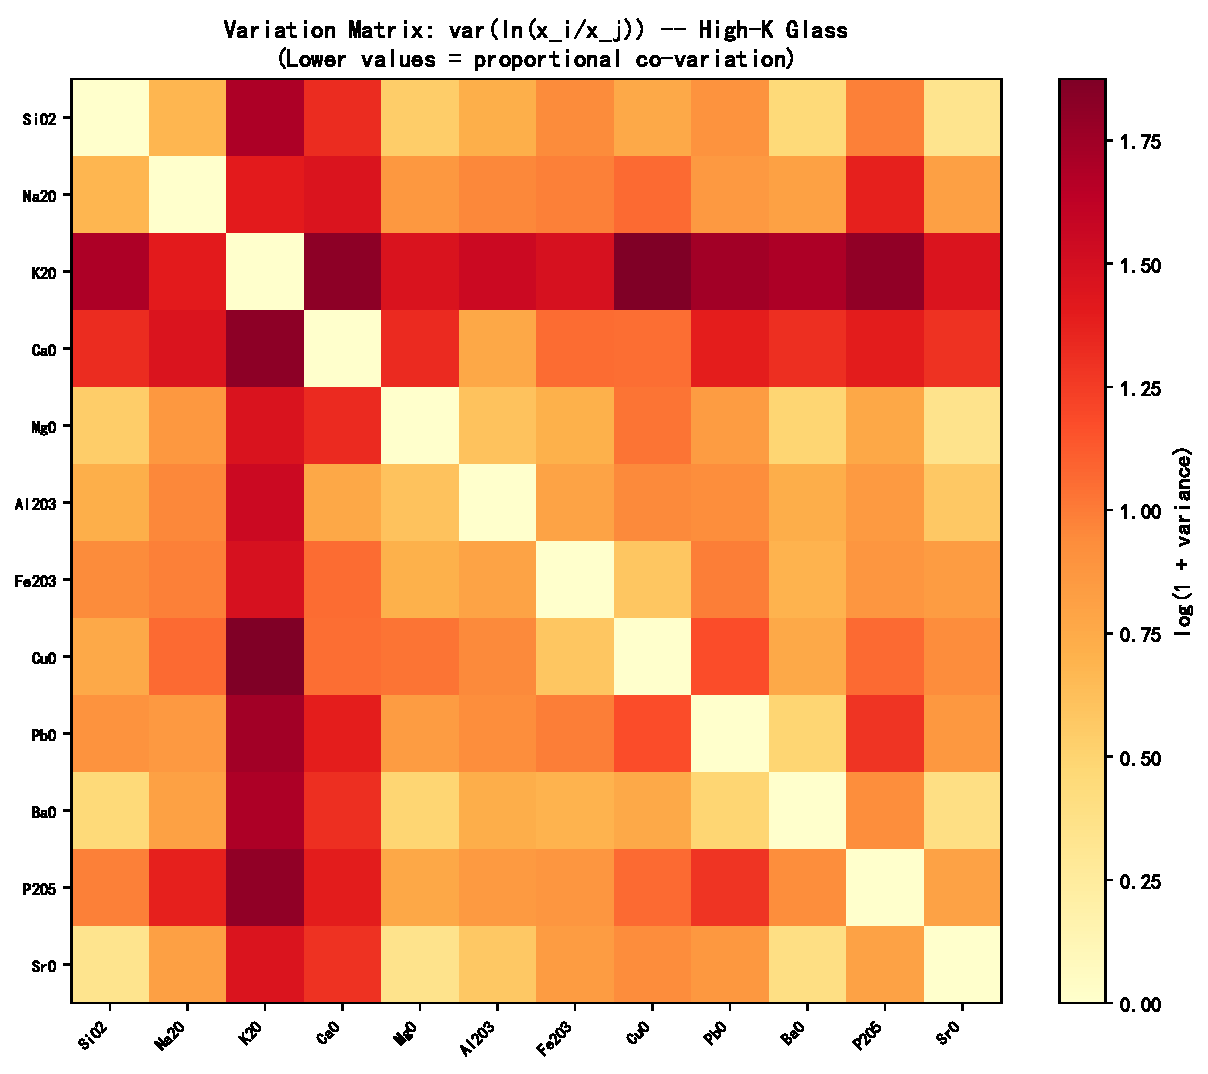
\includegraphics[width=0.48\textwidth]{fig9_high-k_var_matrix.pdf}\hfill
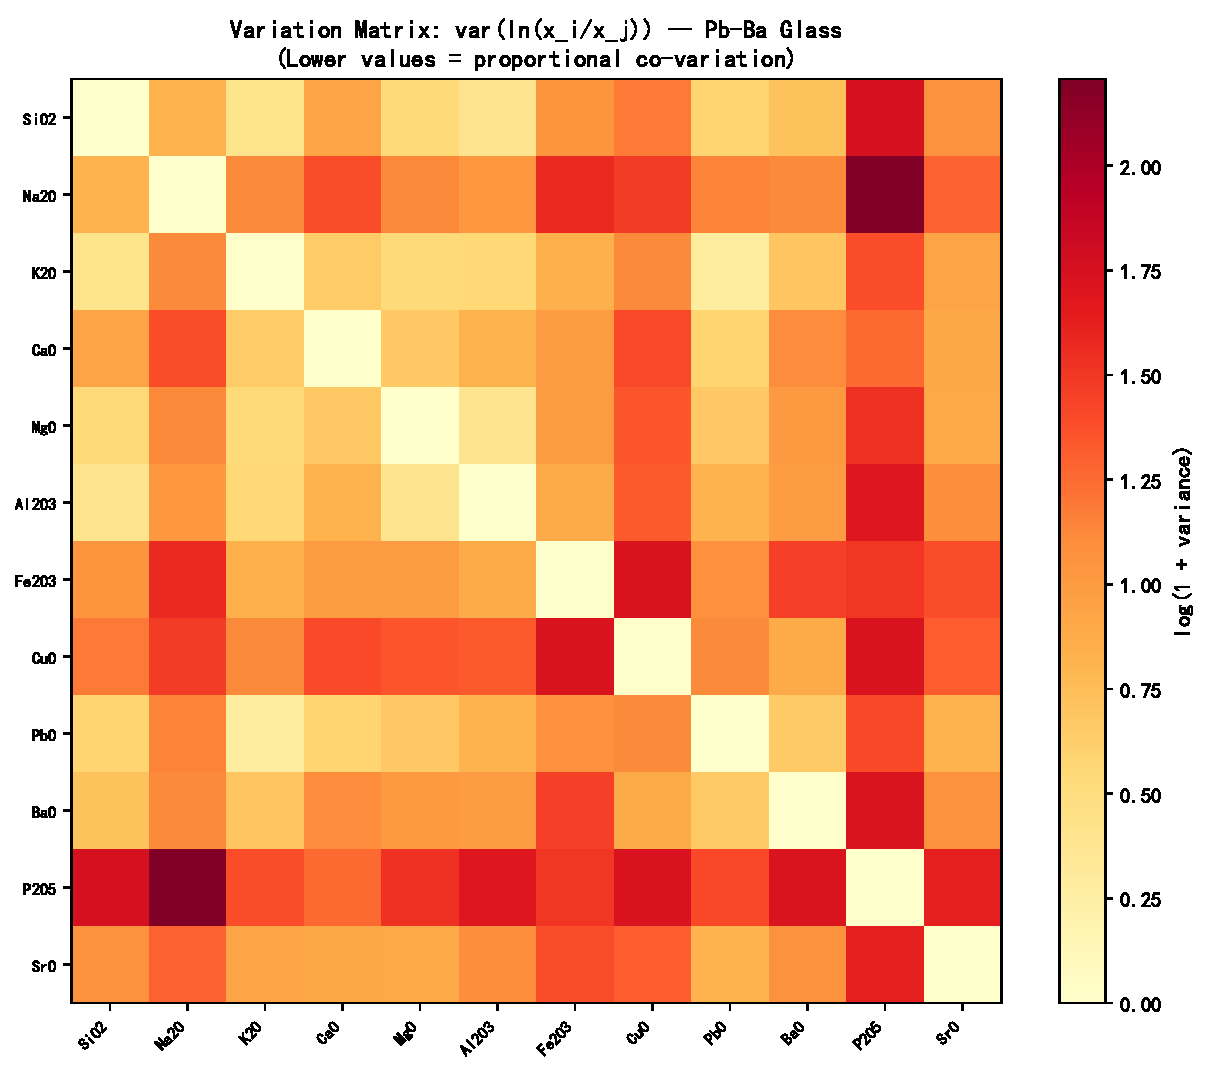
\includegraphics[width=0.48\textwidth]{fig9_pb-ba_var_matrix.pdf}
\caption{高钾玻璃(左)和铅钡玻璃(右)的组成变异矩阵热力图}
\label{fig:var_matrix}
\end{figure}

图\ref{fig:var_matrix}显示两种玻璃类型的变异矩阵呈现显著不同的模式：
\begin{itemize}
    \item \textbf{高钾玻璃}：K$_2$O与其他多数成分的$\tau_{ij}$值较大，表明K$_2$O含量独立于其他元素，这可能反映了草木灰作为独立助熔剂加入时的批次差异。
    \item \textbf{铅钡玻璃}：PbO与BaO之间的$\tau_{ij}$值极小(深色区域)，表明两者存在极强的比例关系，这与铅矿石中Pb和Ba的地球化学共生关系一致。PbO/BaO比值在不同亚类之间存在系统性偏移，可能指向不同铅矿源区。
\end{itemize}

\subsection{关联结构差异检验}

采用排列检验(permutation test)检验两组玻璃的CLR相关矩阵是否存在显著差异：

\begin{equation}
H_0: \Sigma_{\text{高钾}} = \Sigma_{\text{铅钡}}, \quad T = \|\hat{\Sigma}_{\text{高钾}} - \hat{\Sigma}_{\text{铅钡}}\|_F
\end{equation}

将玻璃类型标签随机置换5000次，每次计算置换后的矩阵差的Frobenius范数，构建零分布。

\begin{table}[H]
\centering
\caption{排列检验结果}
\begin{tabular}{c|c|c}
\toprule
\textbf{观测统计量$T_{\text{obs}}$} & \textbf{置换次数} & \textbf{$p$值} \\
\midrule
4.514 & 5000 & \textbf{0.0032} \\
\bottomrule
\end{tabular}
\end{table}

$p=0.0032 < 0.01$，拒绝H$_0$，表明高钾玻璃和铅钡玻璃的化学成分关联结构存在\textbf{极显著差异}。这一结果具有明确的考古学含义：两种玻璃采用了完全不同类型的助熔剂(草木灰 vs 铅矿石)，导致其化学成分的共变模式呈现截然不同的特征。

\subsection{PCA双标图可视化}

\begin{figure}[H]
\centering
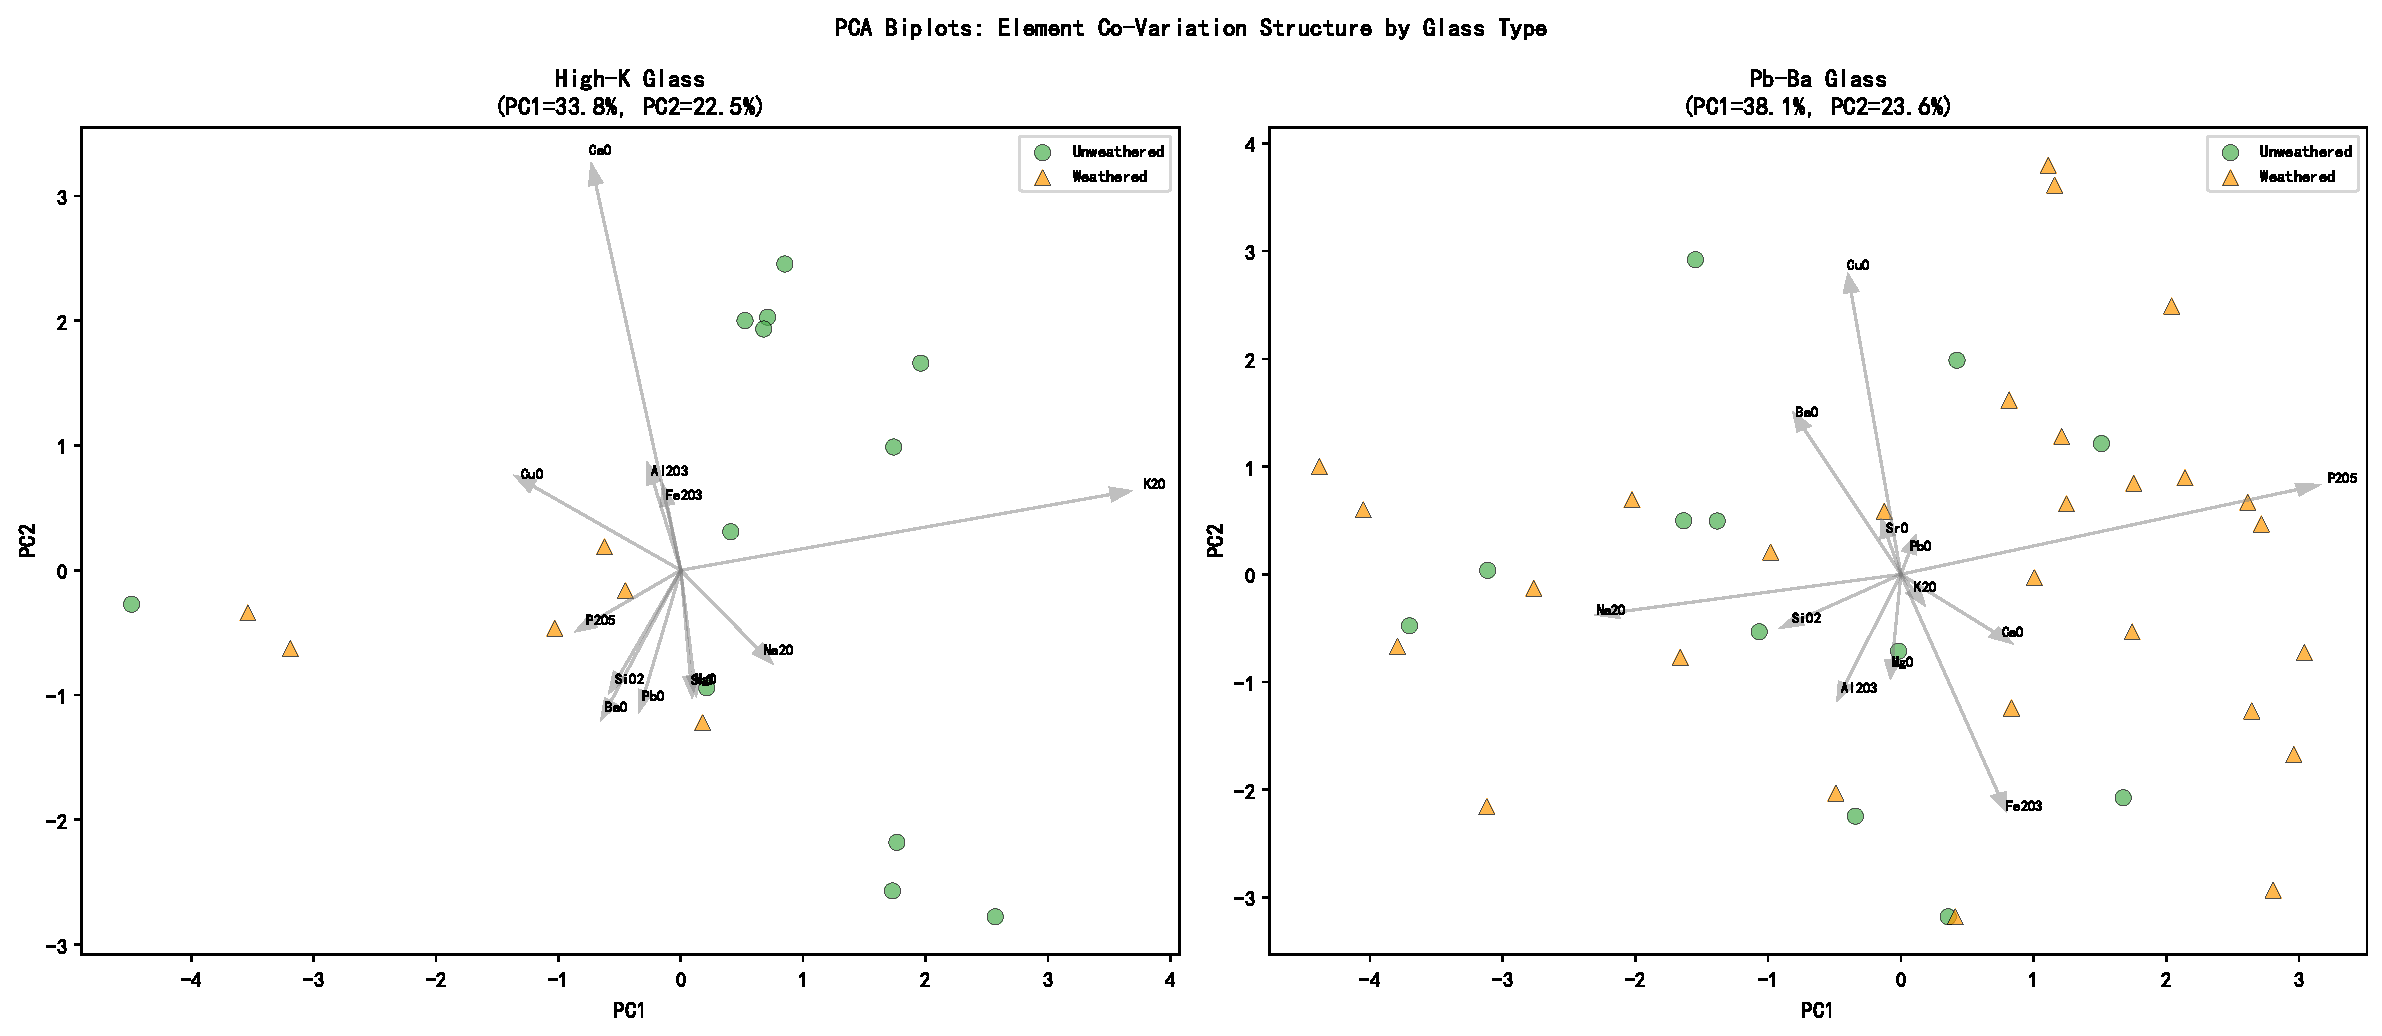
\includegraphics[width=0.95\textwidth]{fig10_pca_biplots.pdf}
\caption{高钾玻璃(左)和铅钡玻璃(右)的PCA双标图。箭头方向表示各元素在主成分空间中的载荷}
\label{fig:pca_q4}
\end{figure}

从图\ref{fig:pca_q4}中可以清晰观察到：
\begin{itemize}
    \item \textbf{高钾玻璃}：第一主成分(PC1，解释方差$>40\%$)主要由K$_2$O与SiO$_2$的对立关系驱动——当K$_2$O含量高时SiO$_2$含量降低，这正是添加草木灰助熔剂降低石英砂比例在成分空间中的体现。
    \item \textbf{铅钡玻璃}：风化与未风化样本在PCA空间中形成两个可分辨的簇，与Q1B中识别的风化效应一致。PbO和BaO的载荷向量近乎平行，再次验证了两者的共变关系。
\end{itemize}

\section{模型评价与改进}

\subsection{模型优势}

\begin{enumerate}[label=\textbf{(\arabic*)}]
    \item \textbf{组成数据处理严谨}：全文统一采用CLR变换处理组成数据，避免了在原始重量百分比上进行相关分析和聚类导致的虚假负相关和偏差。
    \item \textbf{多方法共识验证}：在判别元素识别、亚类划分和未知分类中均采用了多方法交叉验证策略，避免了单一方法的局限性。
    \item \textbf{敏感性分析完备}：对分类结果进行Bootstrap稳定性检验和输入扰动测试，对关联结构采用排列检验，所有关键结论均有定量不确定性评估。
    \item \textbf{考古学可解释性}：所有统计分析结果均与考古化学知识进行对照解释(PbO-BaO共生、K$_2$O与草木灰的关系、Al$_2$O$_3$的化学惰性等)。
\end{enumerate}

\subsection{模型局限与改进方向}

\begin{enumerate}[label=\textbf{(\arabic*)}]
    \item \textbf{样本量不均衡}：高钾玻璃仅有18件，亚类4仅含4个样本，小样本亚类的统计推断不确定性较大。未来可通过更多考古采样扩大高钾玻璃数据集。
    \item \textbf{风化校正模型}：基于Al$_2$O$_3$不移动假设的归一化模型虽具有物理基础，但未能考虑多元素协同迁移的复杂风化机制。若有更多配对风化/未风化数据，可建立多元回归校正模型。
    \item \textbf{检出限问题}：Na$_2$O在高钾玻璃中的系统性缺失(低于检出限)限制了其在判别和聚类中的使用。更先进的左截断统计方法(如Kaplan-Meier型估计)可能进一步改善小样本下的推断。
    \item \textbf{时空信息的缺乏}：数据集中无文物出土地点和年代信息，限制了对亚类化学差异的考古学解释深度。
\end{enumerate}

\section{结论}

本文针对古代玻璃制品的成分分析与鉴别，建立了从风化分析、分类规律发现、未知样品鉴别到成分关联挖掘的完整统计建模框架。主要结论如下：

\textbf{(1)} 玻璃风化与玻璃类型和纹饰类型存在显著统计关联(卡方检验$p<0.03$)。风化导致K$_2$O、SiO$_2$等主要成分的显著变化，变化模式因玻璃类型而异。

\textbf{(2)} PbO、BaO、K$_2$O是区分高钾玻璃和铅钡玻璃的关键判别元素。两种玻璃可进一步划分为2个(高钾)和4个(铅钡)化学亚类，聚类结果具有良好的Bootstrap稳定性。

\textbf{(3)} 8件未知文物中，A1、A6、A7为高钾玻璃，A2--A5、A8为铅钡玻璃。分类结果在$\pm5\%$扰动下保持98\%的稳定性。

\textbf{(4)} 高钾玻璃和铅钡玻璃的化学成分关联结构存在极显著差异(排列检验$p=0.0032$)，反映了两种玻璃在助熔剂选择和制作工艺上的本质区别。

综上，本文的建模方法为考古化学中的玻璃文物分类提供了严谨的统计学工具，对理解古代玻璃制作技术的传播和演变具有参考价值。

\begin{thebibliography}{99}
\bibitem{aitchison1986} Aitchison, J. (1986). \textit{The Statistical Analysis of Compositional Data}. Chapman \& Hall.
\bibitem{pawlowsky2015} Pawlowsky-Glahn, V., Egozcue, J.J., \& Tolosana-Delgado, R. (2015). \textit{Modeling and Analysis of Compositional Data}. Wiley.
\bibitem{henderson2000} Henderson, J. (2000). \textit{The Science and Archaeology of Materials}. Routledge.
\bibitem{gan2009} 干福熹等 (2009). 中国古代玻璃的起源——中国最早的古代玻璃研究. \textit{中国科学E辑}, 39(1), 109-120.
\bibitem{gan2016} 干福熹 (2016). 中国古代玻璃技术的发展. \textit{自然杂志}, 38(1), 19-28.
\bibitem{filzmoser2018} Filzmoser, P., Hron, K., \& Templ, M. (2018). \textit{Applied Compositional Data Analysis}. Springer.
\bibitem{breiman2001} Breiman, L. (2001). Random Forests. \textit{Machine Learning}, 45(1), 5-32.
\end{thebibliography}

\newpage
\section*{附录：主要代码文件}

本文所有分析和图表由Python实现，主要依赖numpy、scipy、pandas、scikit-learn、matplotlib和seaborn。完整可复现代码见\texttt{code/run\_all.py}。关键结果汇总于\texttt{results/RESULTS\_MANIFEST.json}(69项记录)。

\end{document}
